\documentclass[12pt, a4paper]{article}
\setlength{\headheight}{20pt}
%\renewcommand{\baselinestretch}{1.5}
\usepackage[margin=3cm]{geometry}
\usepackage{setspace}
%\onehalfspacing
\setstretch{1.2}
%\usepackage{mathptmx}% Times Roman font
%\usepackage{utopia}
%\usepackage{newcomputermodern}
\usepackage{lmodern}
\usepackage{amsmath}
\usepackage{amssymb}
\usepackage{mdframed}
\usepackage[T1]{fontenc}
\usepackage{fancyhdr}
\usepackage{pgfplots}
\usepackage{csquotes}
\newcommand\s{30} %samples i grafer. set til 1000, 80 for arbejde
%\newcommand{\doubleunderline}{\underline{\underline{}}}
\usepackage{lipsum}
\usepackage{blindtext}
%flyta myndir
\usepackage{graphicx}
\usepackage{float}
\usepackage{sidecap}
%flyta myndir end

\usepackage{titlesec}
\titleformat{\section}
{\LARGE \bfseries}
{\thesection}
{1em}
{}

\titleformat{\subsection}
{\large \bfseries}
{\thesubsection}
{0.5em}
{}

%bruka inkscapefílir
\usepackage{import}
\usepackage{xifthen}
\usepackage{pdfpages}
\usepackage{transparent}

\newcommand{\incfig}[1]{%
    \def\svgwidth{6.00cm}
    \import{./figures/}{#1.pdf_tex}
}
\renewcommand*\contentsname{Indholdsfortegnelse}
\renewcommand{\figurename}{Figur}
%bruka inkscapefílir end

\makeatletter
\patchcmd{\csq@bquote@i}{{#6}}{{\emph{#6}}}{}{}
\makeatother



%\usepackage[backend=biber,sorting=nty,style=verbose]{biblatex}
\usepackage[backend=biber,sorting=nty, style=authoryear-ibid]{biblatex}
\addbibresource{bibliografi.bib} %Imports bibliography file
\DeclarePrintbibliographyDefaults{heading=none}
\title{Taylorpolynomier}
%\author{Jákup H. Lützen}
\date{Februar 2022}
%\pagestyle{fancy}
%\fancyhead{}
%\fancyfoot{}
\begin{document}
\begin{titlepage}
   \centering
    \vfill
%    \maketitle
    {\huge 
    Taylorpolynomier\\
    \vspace{0.5cm}
    \large
    SSO - Matematik A\\
    \vspace{0.25cm}
    Februar 2022
    }    
    \vfill
%    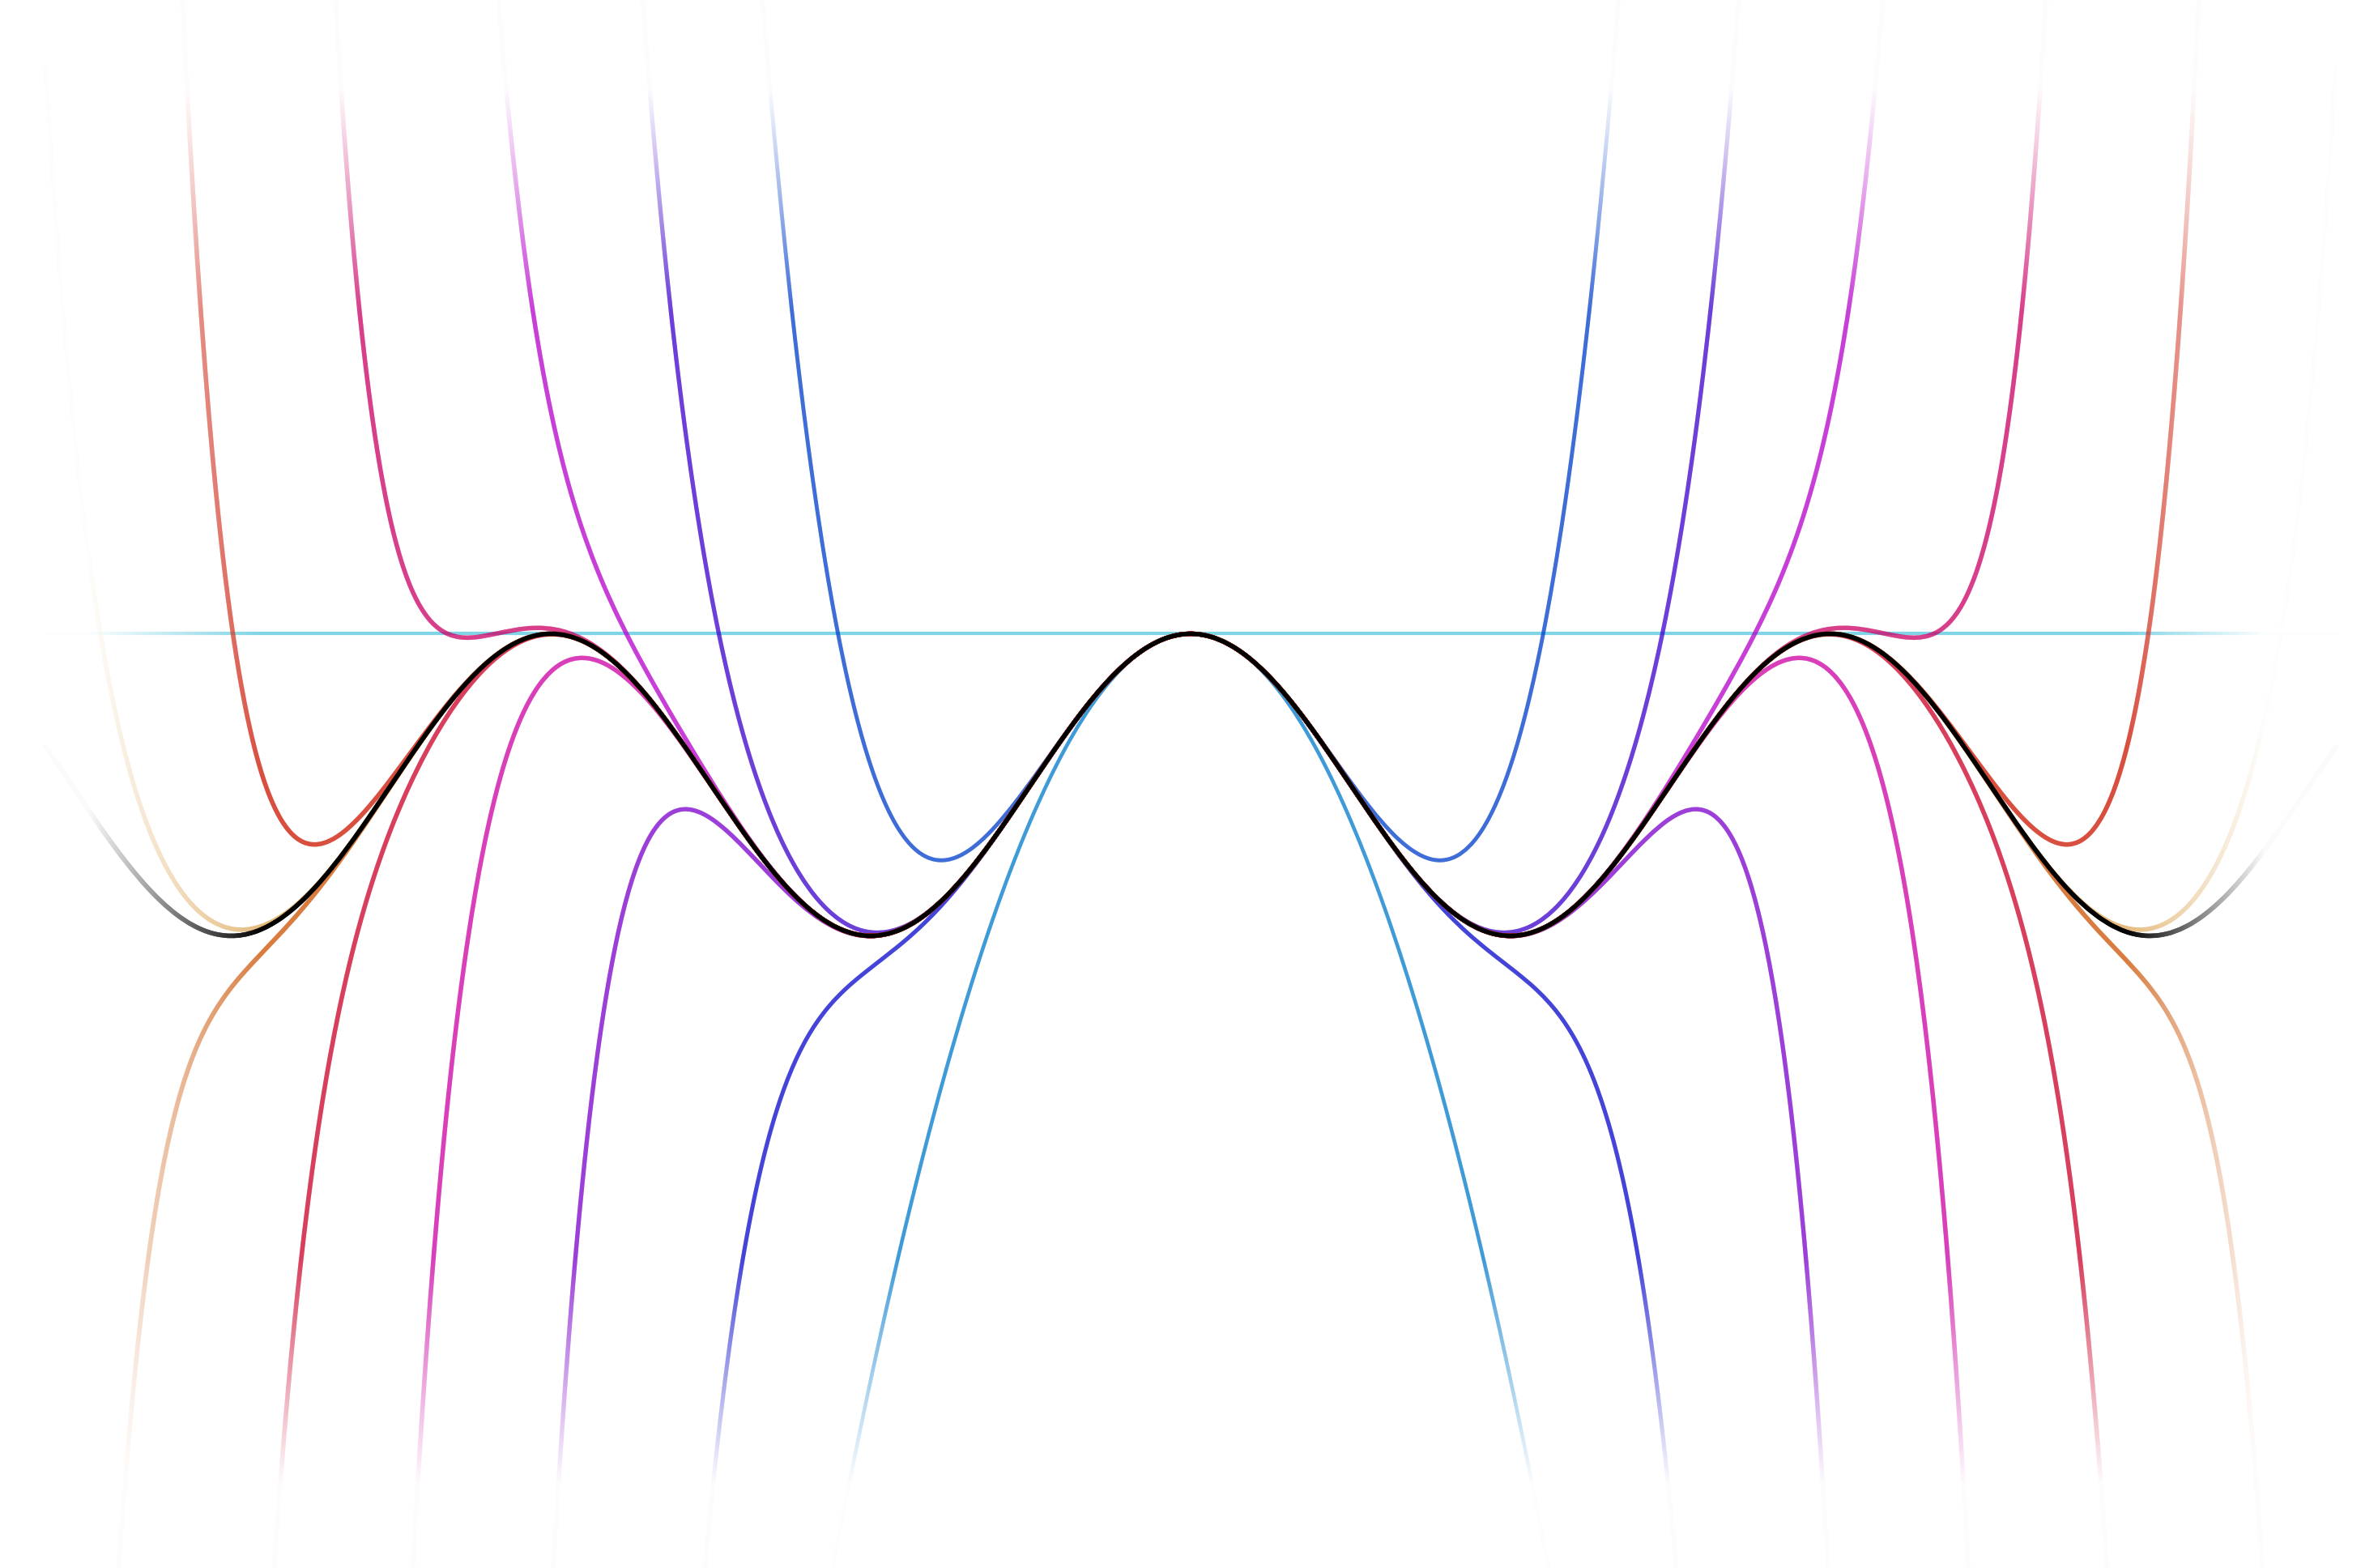
\includegraphics[width=\textwidth]{figures/forside3edit2.png} % also works with logo.pdf
   
    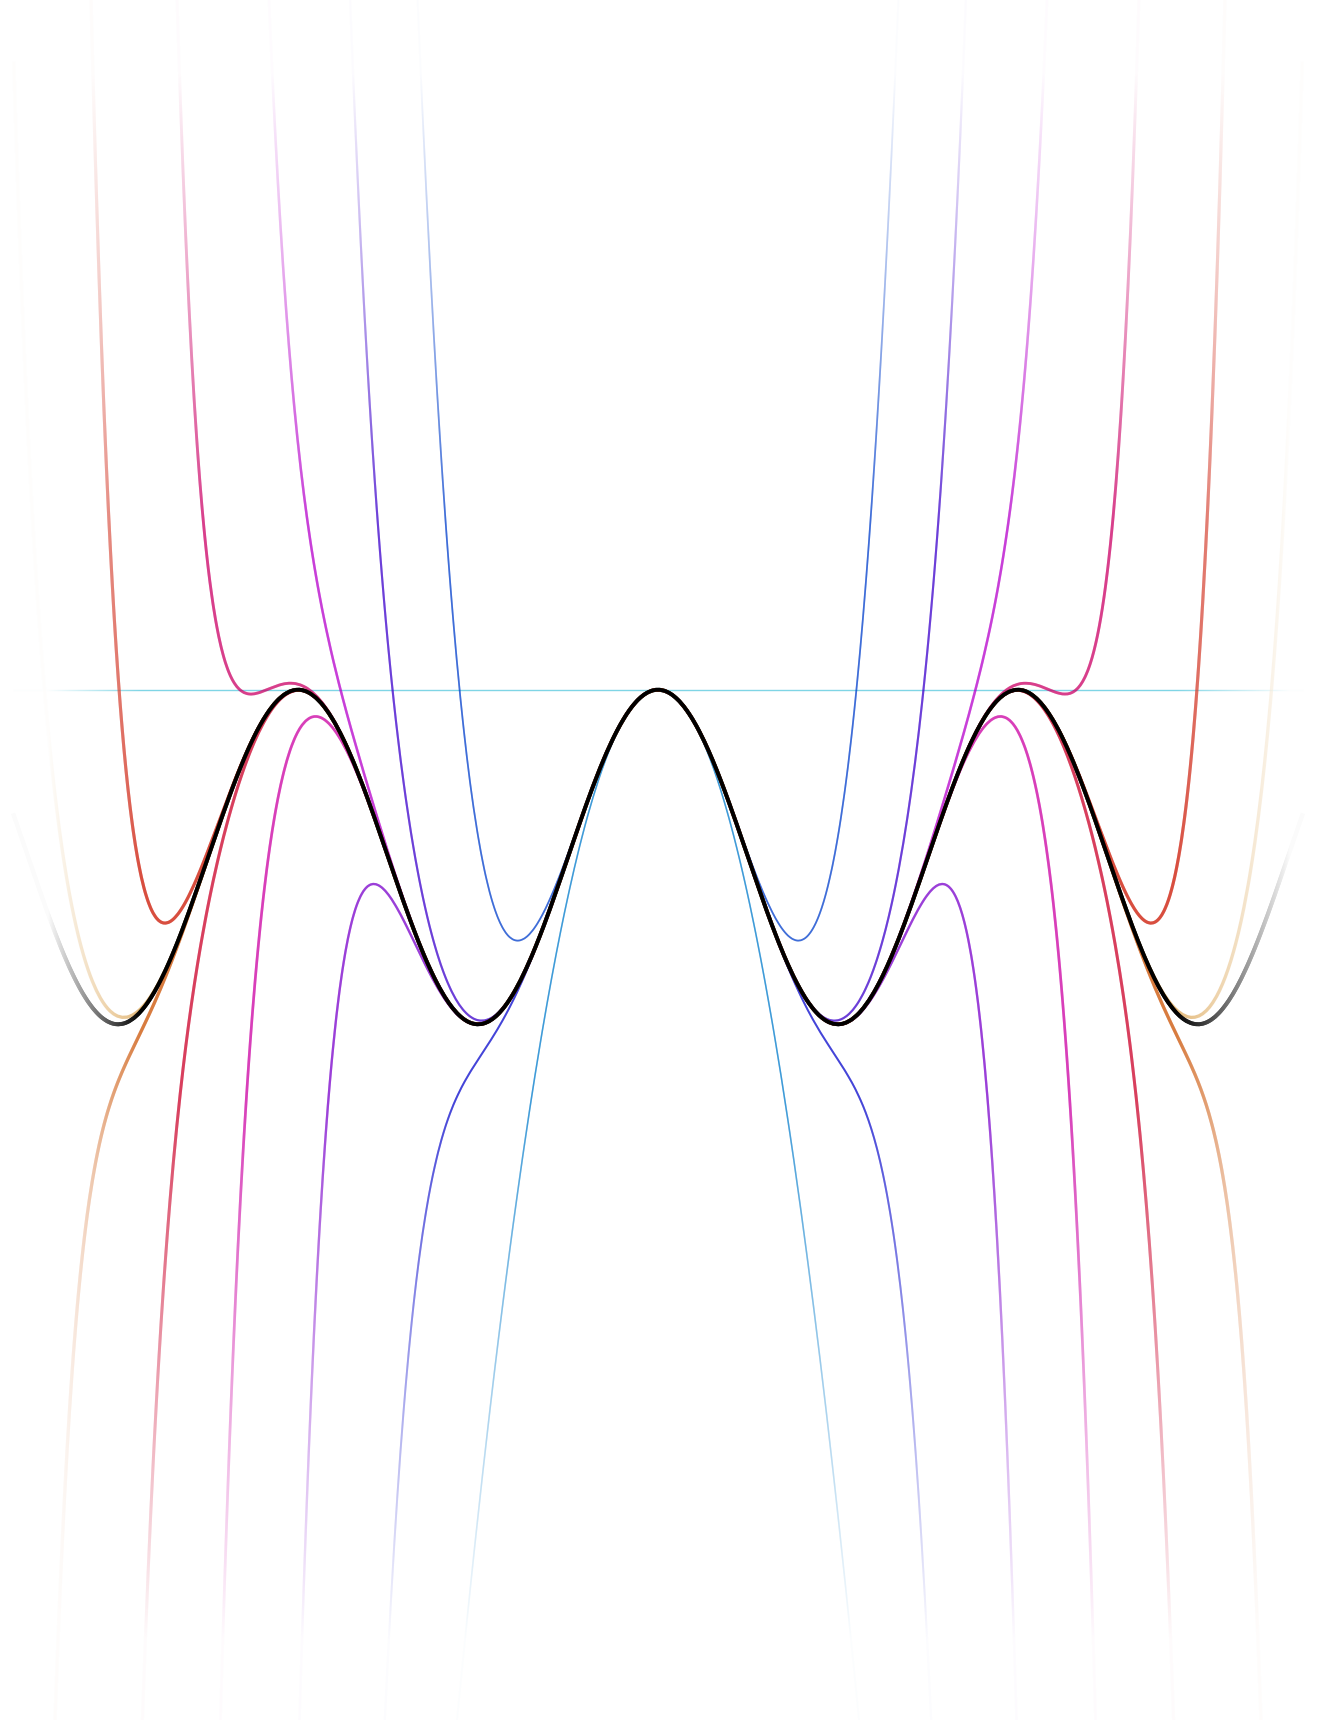
\includegraphics[width=\textwidth]{figures/forside4edit.png} % also works with logo.pdf
    \vfill
    \vfill
\thispagestyle{empty}

\end{titlepage}
%%%%% \footnote{hey} fyri vanligan footnote
%%%%%\footcite{talogrækker} fyri referencu
%%%%% :set spell spelllang=da (fyri at byrja spellcheck)
%%%% :set nospell fyri at sløkkja
%\setcounter{page}{2} % Set dette hvis første side tæller med i sidecount 
\section*{Resume} %150 ord (det essentielle i min opgave, dvs ca 8 linjer
\blindtext[1-2]
\tableofcontents
\newpage



\section{Indledning} %ca en halv side til en side. I egne ord, hvorfor dette er interessant. God ide at slutte af med problemformuleringen, "Og her vil jeg..."
Matematik kan til tider synes firkantet og rigidt, hvor abstrakte forhold opskrives i eksakte formler, og hvor der ikke er plads til kreativitet. 
Dykker man dybere ind i faget vil man dog opdage, at dette ikke er tilfældet, og at der er mange situationer, hvor man gør kreativt brug af relativt ueksakte værktøjer. Et af disse er såkaldte Taylorpolynomier.


I matematikkens verden findes der alverdens slags funktioner, hvor nogle er mere medgørlige end andre. Nutidens computerteknik kræver desuden hurtig og praktisk behandling af alle disse formler, og i den forbindelse indtræder Taylorpolynomier ofte.\\
\\
Taylorpolynomier er ingen ny opfindelse. De dukkede for første gang op i 17-18. århundrede, men hvordan blev de opdaget? Der er ingen tvivl om at de har haft stor indflydelse på måden som matematik bliver behandlet i dag, men hvordan ved man om de er korrekte, i hvilken grad ved man det, og hvorfor er det i det hele taget relevant i dag?\\
\\
Denne opgave vil beskrive den historiske baggrund for Taylorrækken, bevise formlen for Taylorrækken, undersøge dens restled, samt undersøge hvilke praktiske anvendelser Taylorpolynomier har i dag.

\section{Taylorrækkens historie} % Redegørelse Egne ord. Ikke inddrage citater (fordi så bliver det analyserende).
Matematikeren Brook Taylor (1685 - 1731) er navnefader til hvad vi i dag kalder Taylorpolynomier, efter at han i 1715 offentliggjorde en generel formel for principperne.
Taylors formel ser således ud i sin moderne form:\footcite[s. 247]{roy_2021}
\begin{equation*}
   f(x)=f(a)+f(x-a)\frac{f'(a)}{1!}+(x-a)^2\frac{f''(a)}{2!}+\cdots. 
\end{equation*}
Dette kan naturligvis også skrives som:
\begin{equation*}
    f(x)=\sum_{n=0}^{\infty}\frac{f^{(n)}(a)}{n!}(x-a)^n.
\end{equation*}
Men Taylor var dog ikke den første der tænkte disse tanker.
\subsection{Newton, Gregory og Bernoulli}

Taylorpolynomier bygger på en indseelse, at der er en forbindelse mellem en funktions koefficienter og dens afledte. Denne indseelse viser Isaac Newton (1643 - 1727) for første gang i hans \textit{Principia} (1687), og få år senere giver han et egentligt eksempel af Taylors formel i sin \textit{De Quadratura Curvarum} (1691 - 92), som han aldrig færdiggjorde. Dele af denne tekst blev udgivet med titlen \textit{Tractatus de Quadratura Curvarum}, men Taylors formel blev desværre udladt.\footcite[s. 248]{roy_2021} Newton havde altså opdaget disse samme principper femogtyve år tidligere end Taylor, uden at de blev udgivet.\\
\\
Newton havde i det hele taget svært ved at udgive sine findelser før han blev kendt i videre kredse, hvilket til tider voldte ham problemer i at blive anerkendt for sine opdageser. \footcite[s. 116]{uendeligerækker}\\
En af konsekvenserne af dette var den kendte kontroversi imellem Newton og Gottfried Wilhelb Leibniz (1646 - 1716), da de ifølge Mejlbo:
\blockquote{blev indviklede i en ulykkelig strid om ophavsretten til differential- og integralregningen. Den gik værst  ud over Leibniz. Royal Society dømte ham - ganske uberettiget - for plagiat}.\footcite[s. 103]{uendeligerækker}\\
En af Leibnitz' største fortalere i denne prioritetsstrid var Johann Bernoulli (1667 - 1748), som i slutningen af 1690'erne også havde udgivet en formel der lignede Taylors formel. Mejlbo skriver om Bernoulli at: \blockquote{\dots han havde et voldsomt temperament, så han overfusede Taylor med beskyldninger for plagiat.}\footcite[s. 111]{uendeligerækker}.\\
\\
Den tidligste opdager af Taylors formel var dog nok den Skotske matematiker James Gregory (1638 – 1675).\\
\textcolor{red}{\textbf{Mere om Gregory}} 
\section{Analyse} % Kød og kartofler. Brug modellen (introducere citatet, så kommer citatet, og så kommenterer man.
\subsection{Pædagogisk gennemgang (arbejdstitel)}
Man kan opnå en intuitiv forståelse for Taylorpolynomier med følgende fremgangsmåde:\\
Vi ønsker at approksimere en given funktion fra punktet $x_0$. Den simpleste approksimation kunne være funktionens tangentligning i punktet $x_0$
\begin{figure}
     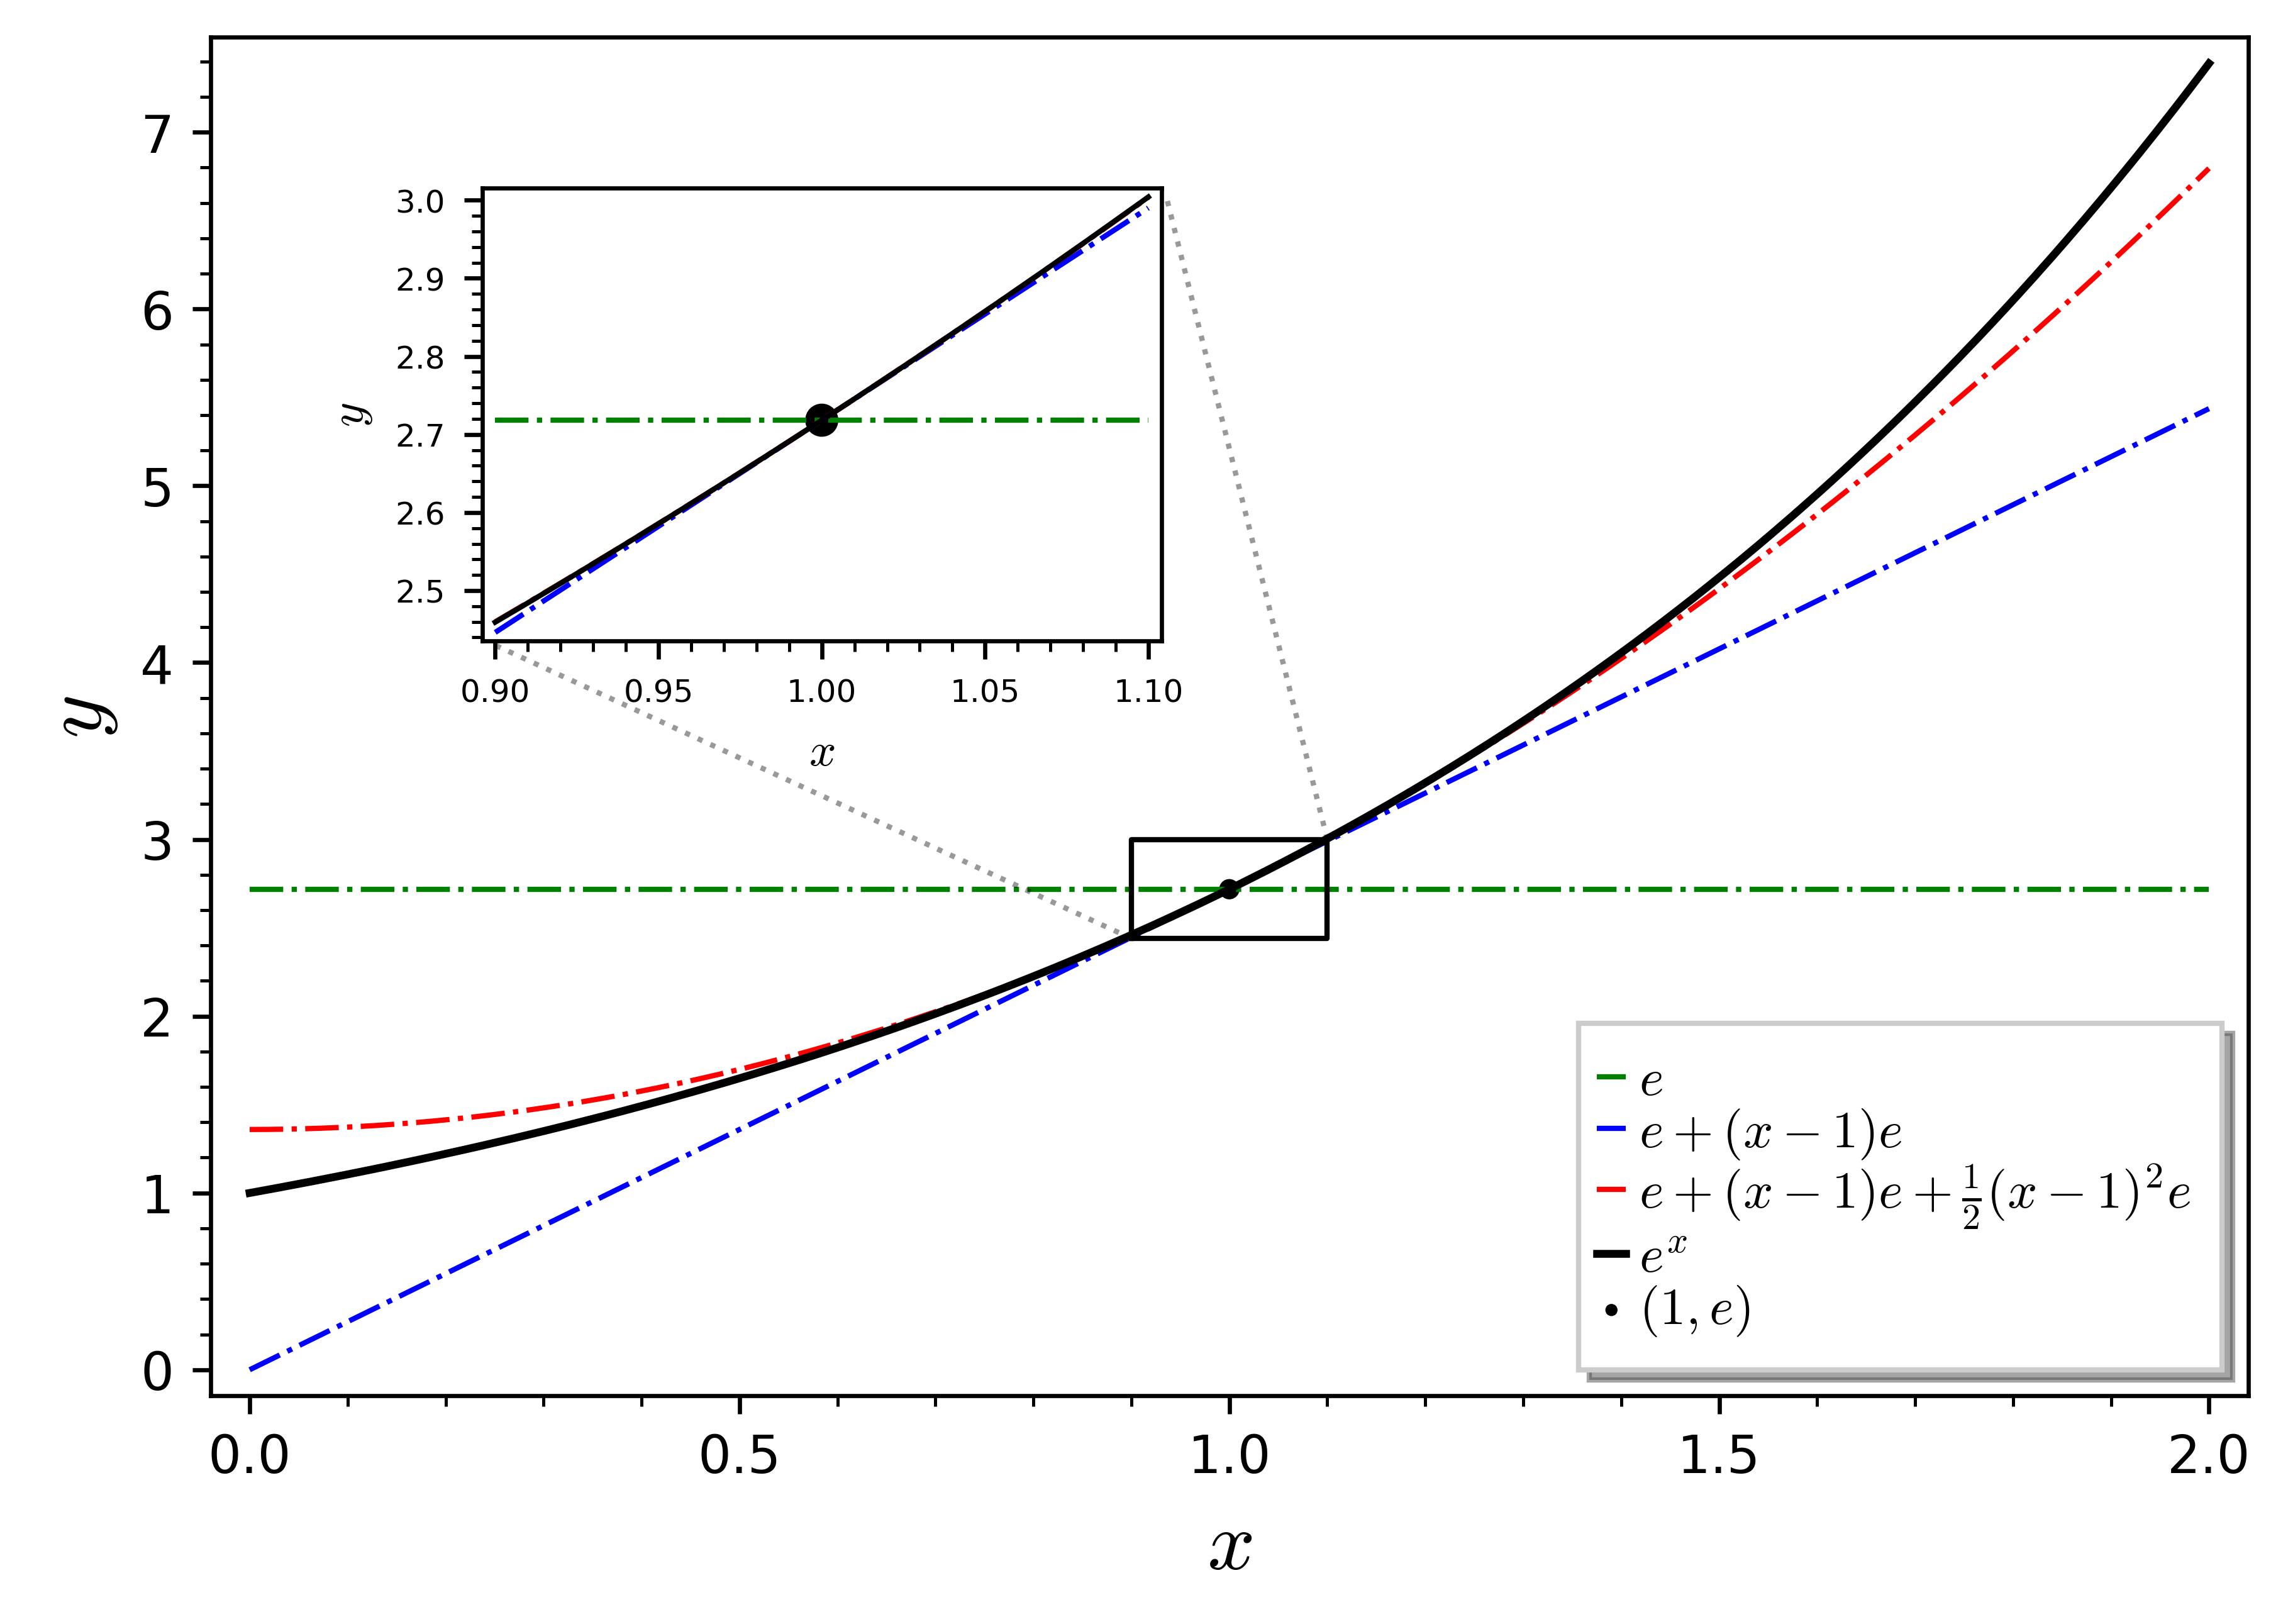
\includegraphics[width=\textwidth]{figures/ex-eksempel.png}
     \caption{Første- anden- og tredjegrads Taylorpolynomium for $e^x$}
     \label{fig:boat1}
\end{figure}
\subsection{Beviser for Taylorpolynomiet}
\section{Diskussion/Vurdering} % Måske tage nogle fagpersoner med eller noget. Gerne selv tage stilling.
\section{Konklusion} % samle problemformuleringens underspørgsmål. "jeg har. og så... jeg kan konkludere..."

\section{Litteraturliste}
%\nocite{*}
\subsection{Referenceliste}
\printbibliography
\subsection{Litteraturliste}
%\printbibliography[keyword=online]
Forsidebillede er skabt af undertegnede.
\end{document}

